\subsection{Wizualizacja}

Widok graficzny aplikacji został zaimplementowany z wykorzystaniem biblioteki \textbf{PyQt} oraz języka \textbf{QML}. Zastosowanie QML pozwoliło na deklaratywne definiowanie modułów wizualnych, co znacząco usprawniło proces projektowania i zarządzania interfejsem użytkownika.

\clearpage

\textbf{Widok główny aplikacji}
\begin{figure}[h!]
    \centering
    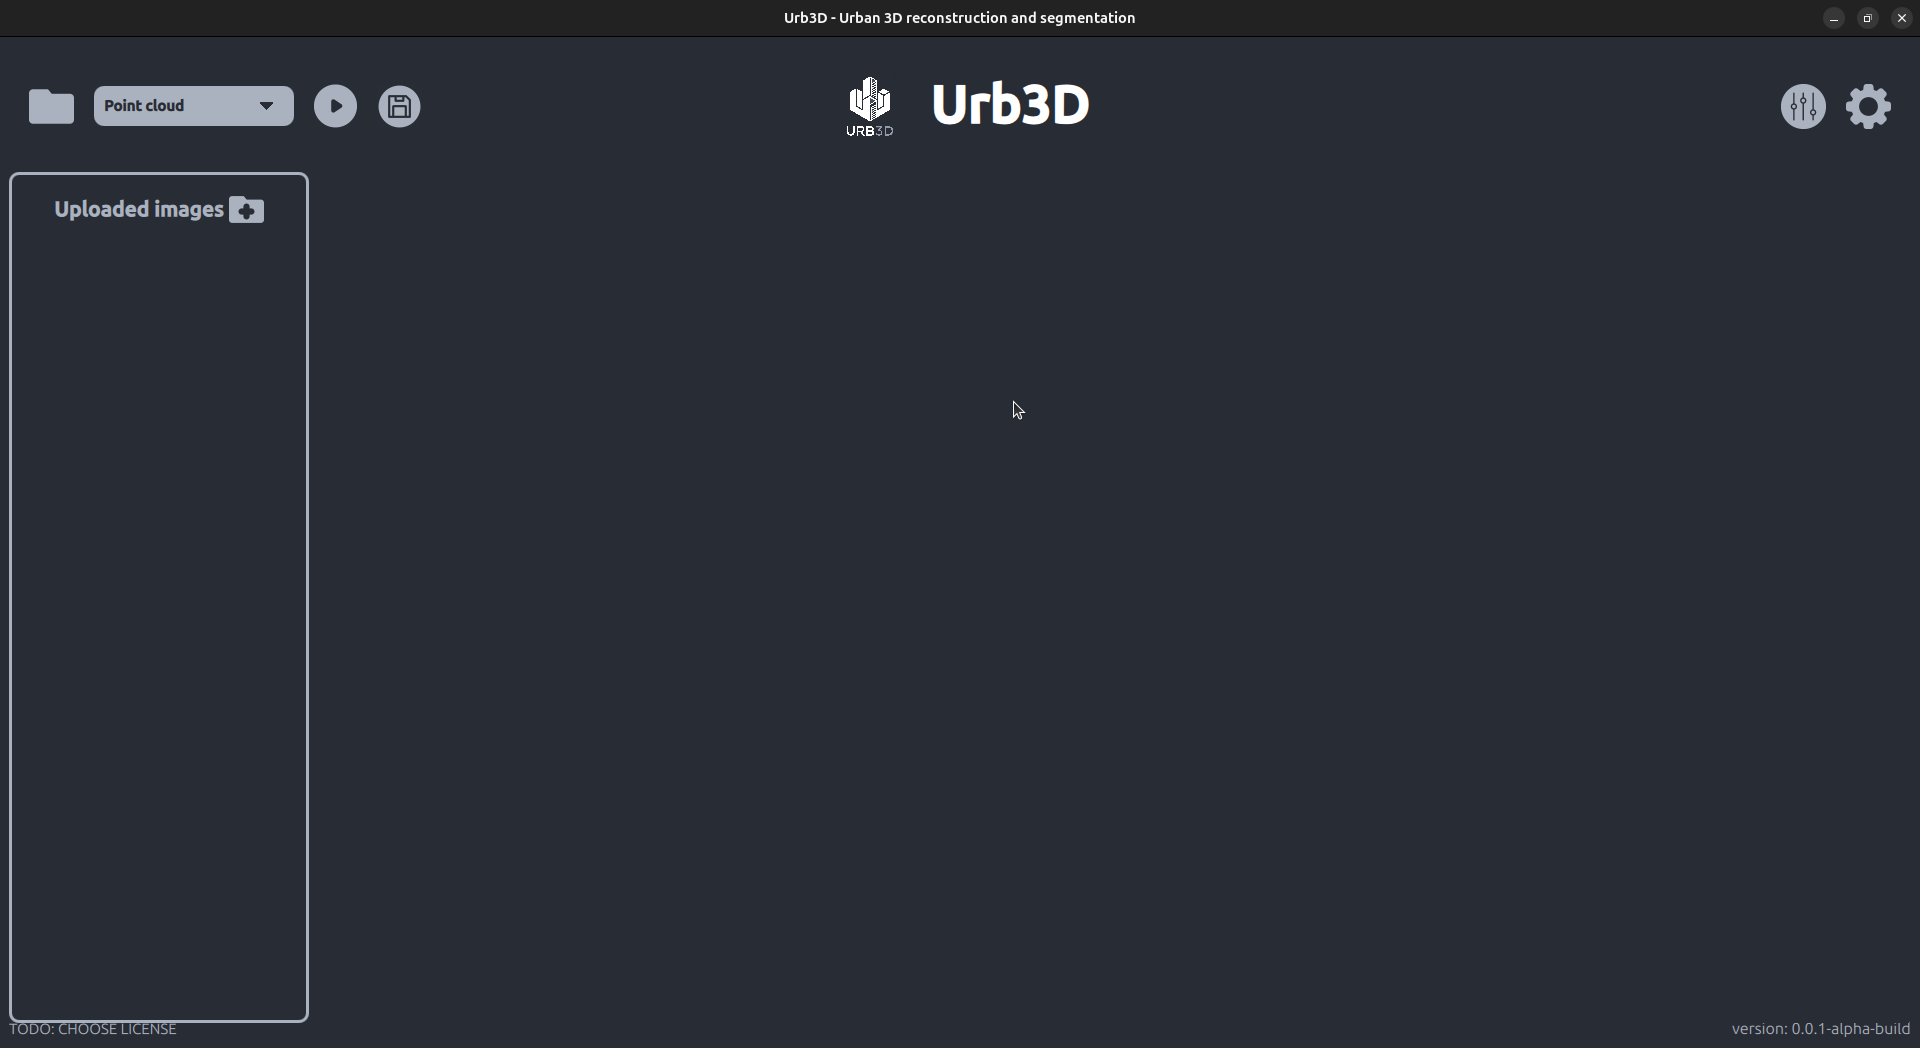
\includegraphics[width=0.8\textwidth]{img/wizualizacja/ui_glowny_widok.png}
    \caption{Widok główny aplikacji.}
\end{figure}

Główny widok aplikacji składa się z trzech kluczowych komponentów:
\begin{enumerate}
    \item \textbf{Pasek zadań (Taskbar)} -- odpowiedzialny za obsługę globalnych akcji i konfiguracji.
    \item \textbf{Panel renderingu (Rendering Panel)} -- obszar przeznaczony do wizualizacji danych renderowanych.
    \item \textbf{Panel zarządzania zdjęciami (Image Management Panel)} -- sekcja umożliwiająca obsługę i manipulację zdjęciami w ramach aplikacji.
\end{enumerate}

\subsubsection{Funkcjonalności paska zadań}
\begin{figure}[h!]
    \centering
    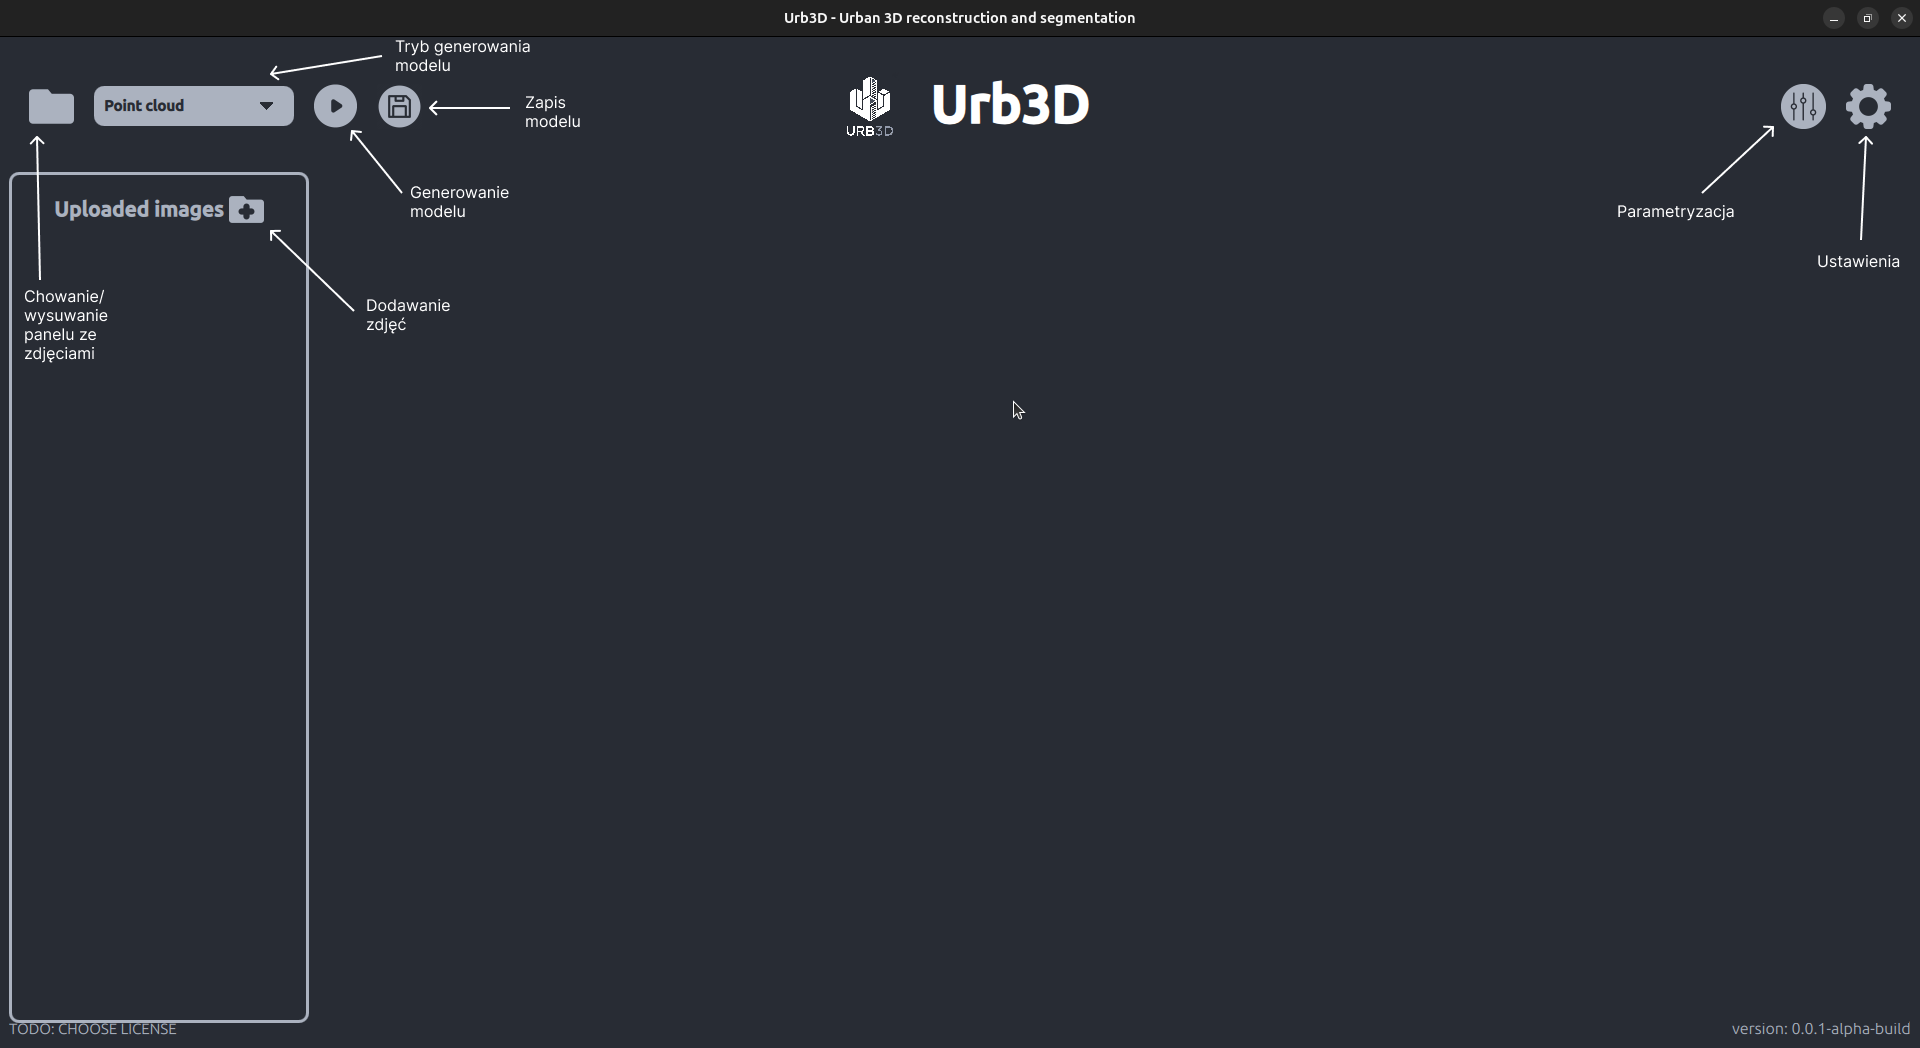
\includegraphics[width=0.8\textwidth]{img/wizualizacja/ui_opis_funk.png}
    \caption{Pasek zadań aplikacji.}
\end{figure}

Pasek zadań zawiera zestaw przycisków umożliwiających użytkownikowi dostosowanie działania aplikacji. 

\textbf{Interakcje użytkownika}
\begin{itemize}
    \item \textbf{Panel renderingu:} możliwość przybliżania, przesuwania i obracania wizualizowanych obiektów za pomocą myszy i klawiszy WASD.
    \item \textbf{Pasek zadań:} przyciski pozwalające na wykonywanie globalnych operacji, takich jak zapisywanie ustawień czy uruchamianie procesów.
    \item \textbf{Panel zarządzania zdjęciami:} dodawanie folderu ze zdjęciami wykorzystywanych do generowania modelu.
\end{itemize}

% \section{Diagram wywołania budowy modelu}
Poniżej przedstawiono diagram wywołania procesu budowy modelu z głównego okna aplikacji. Ilustruje podstawowy przepływ działania aplikacji, tj. tworzenie modelu.

\begin{figure}[h!]
    \centering
    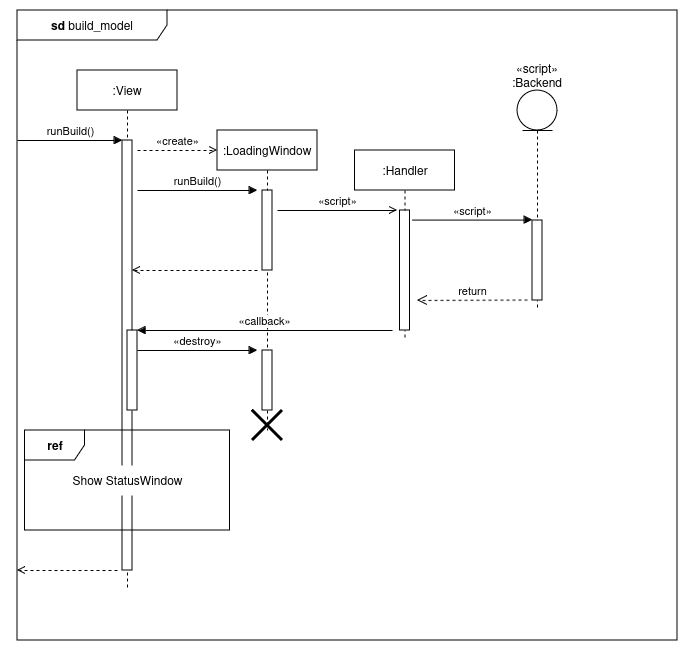
\includegraphics[width=0.8\textwidth]{img/diagramy/diagram_sekw_build.png}
    \caption{Diagram komunikacji między komponentami w trakcie budowy modelu.}
\end{figure}

\subsubsection{Zmiana ustawień aplikacji}
\begin{figure}[h!]
    \centering
    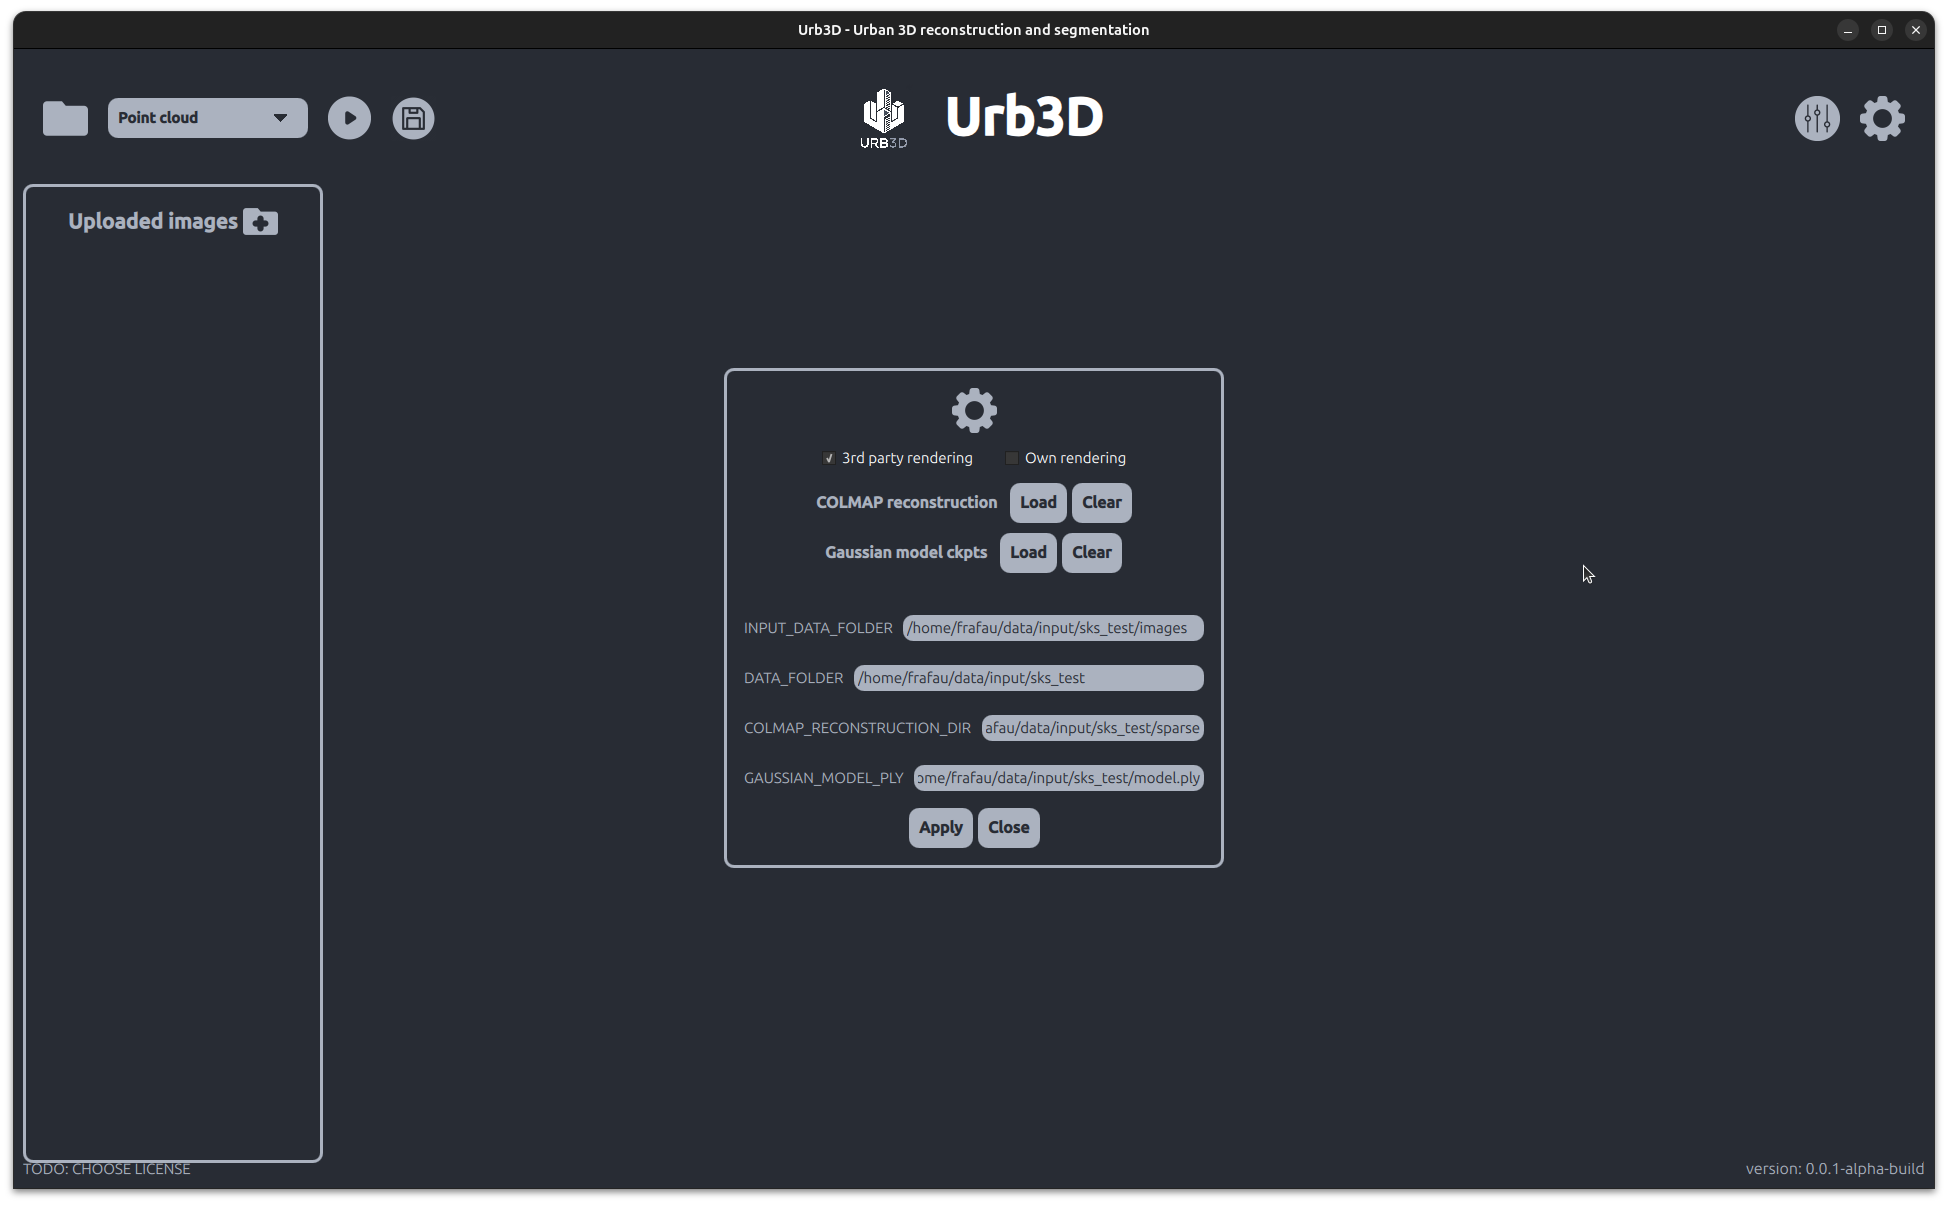
\includegraphics[width=0.8\textwidth]{img/wizualizacja/ui_ustawienia.png}
    \caption{Interfejs zmiany ustawień aplikacji.}
\end{figure}

Funkcja zmiany ustawień pozwala na modyfikację parametrów działania aplikacji, takich jak wybór renderera czy zmiana zmiennych środowiskowych.

\clearpage

\subsubsection{Modyfikacja parametrów}
\begin{figure}[h!]
    \centering
    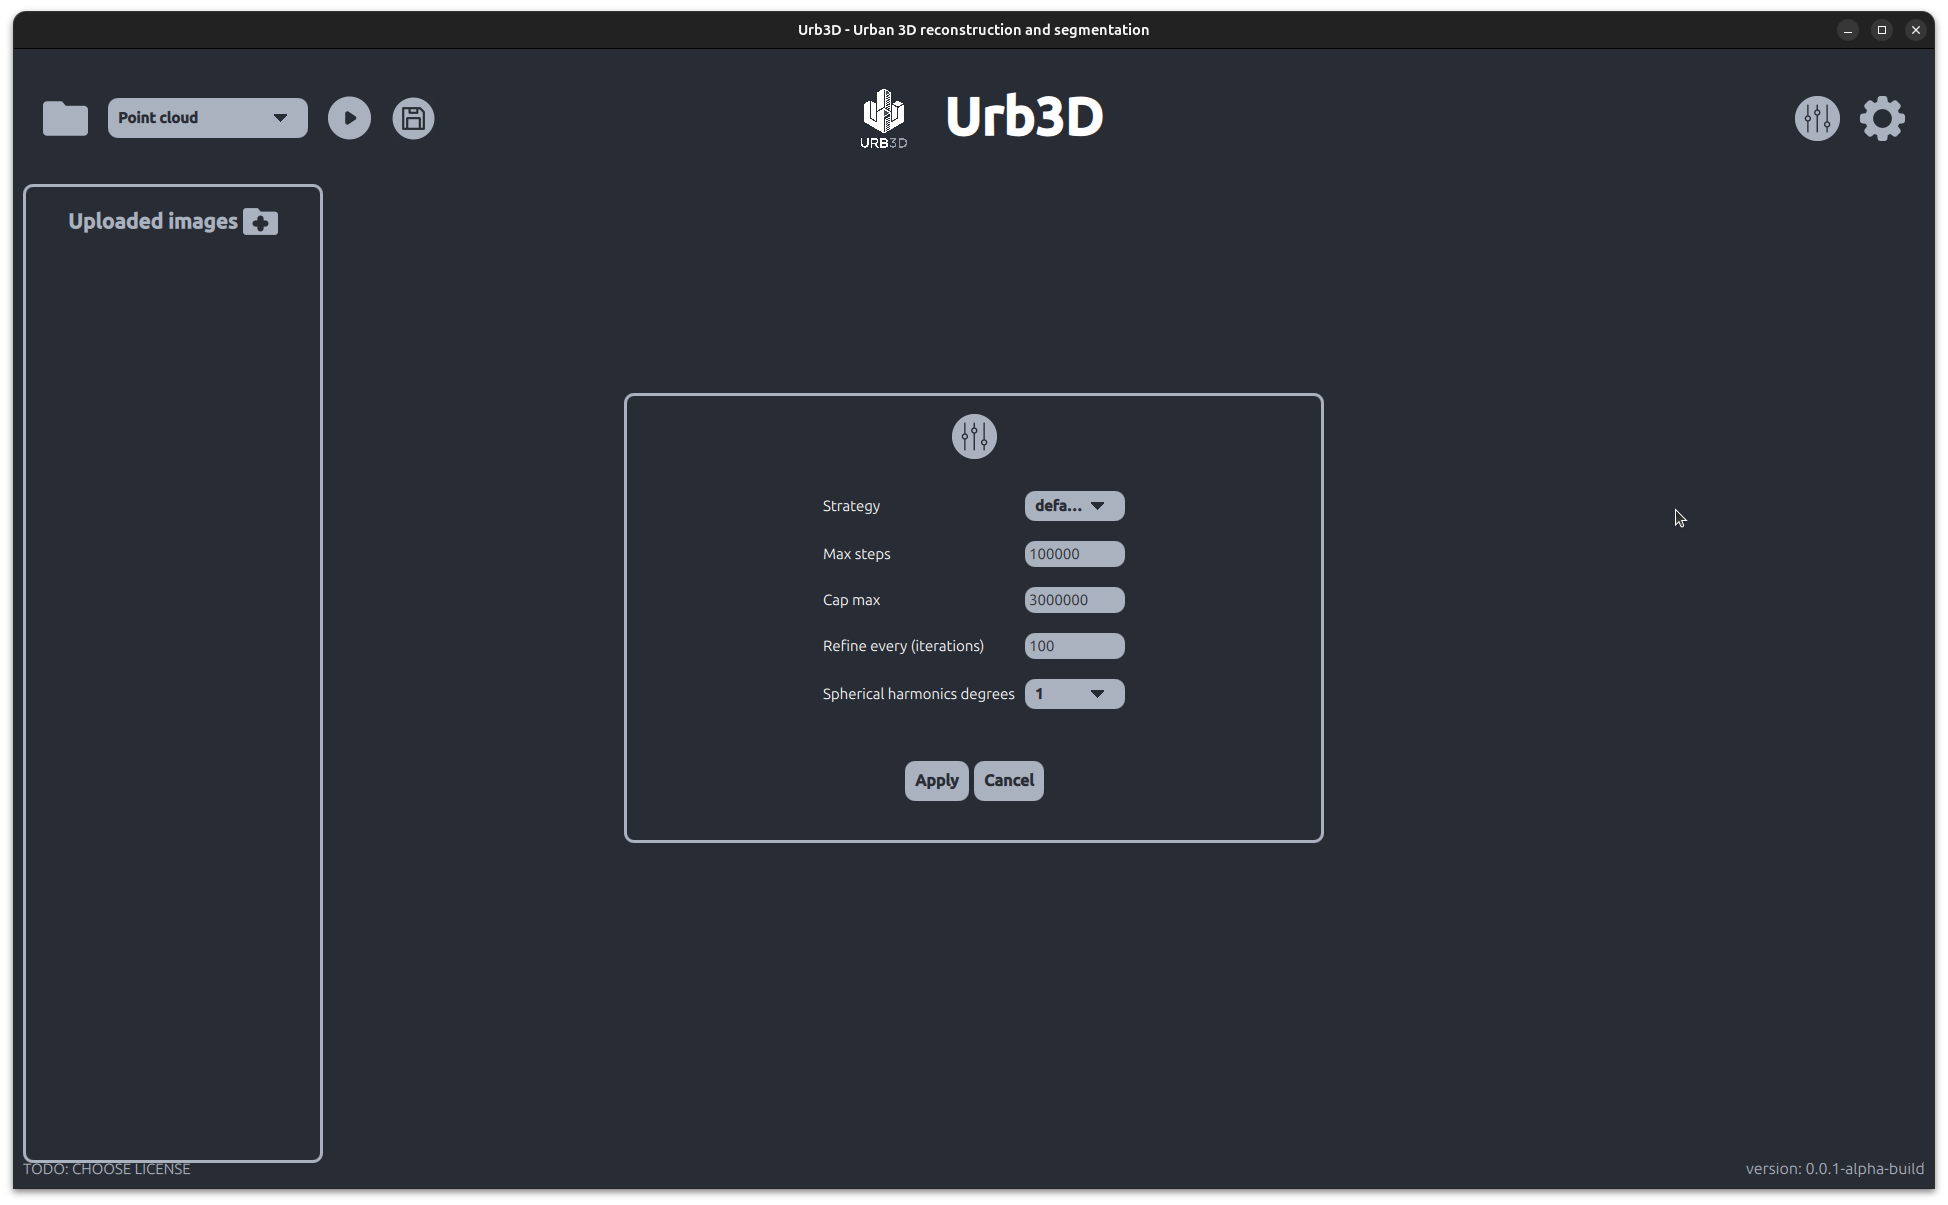
\includegraphics[width=0.8\textwidth]{img/wizualizacja/ui_parametry.png}
    \caption{Interfejs modyfikacji parametrów.}
\end{figure}

Panel parametrów umożliwia dynamiczną zmianę wartości związanych z procesem generowania modelu.

\subsubsection{Podsumowanie sekcji wizualizacji}

Implementacja interfejsu użytkownika z wykorzystaniem PyQt i QML umożliwiła:
\begin{itemize}
    \item szybkie prototypowanie modułów wizualnych,
    \item łatwe modyfikowanie wyglądu i funkcji interfejsu,
    \item zachowanie wysokiej wydajności renderowania dzięki odseparowaniu logiki od widoku.
\end{itemize}

Wizualizacja została zaprojektowana w sposób intuicyjny i modularny, co ułatwia dalszą rozbudowę aplikacji oraz integrację nowych funkcji.
